\documentclass[tikz,border=22pt]{standalone}
\usepackage[T1]{fontenc}
\usepackage{helvet}
\renewcommand{\familydefault}{\sfdefault}
\usepackage{amsmath,amssymb}
\usetikzlibrary{calc,positioning,fit,backgrounds,shapes.geometric,shapes.symbols,arrows.meta,decorations.pathreplacing}

% =============================================================================
% CANONICAL MLSYSBOOK PALETTE
% =============================================================================
\definecolor{DarkSlate}{HTML}{0F172A}
\definecolor{slatesteel}{HTML}{334155}
\definecolor{BlueLine}{HTML}{006395}
\definecolor{BlueL}{RGB}{209,243,255}
\definecolor{BlueL0}{HTML}{F0F9FF}
\definecolor{GreenLine}{HTML}{008F45}
\definecolor{GreenL}{RGB}{219,253,166}
\definecolor{GreenL0}{HTML}{EBF8F2}
\definecolor{forestsage}{HTML}{166534}
\definecolor{OrangeLine}{HTML}{E67817}
\definecolor{OrangeL}{RGB}{254,237,222}
\definecolor{OrangeL0}{HTML}{FFFBEB}
\definecolor{warmochre}{HTML}{92400E}
\definecolor{RedLine}{HTML}{D9534F}
\definecolor{RedL}{RGB}{253,226,240}
\definecolor{RedL0}{HTML}{FEF2F2}
\definecolor{deepburgundy}{HTML}{991B1B}
\definecolor{VioletLine}{HTML}{7E317B}
\definecolor{VioletL}{RGB}{247,215,247}
\definecolor{amethyst}{HTML}{581C87}
\definecolor{amethystL0}{HTML}{FAF5FF}
\definecolor{GrayLine}{HTML}{64748B}
\definecolor{coolparchment}{HTML}{F8FAFC}
\definecolor{CardBorder}{HTML}{CBD5E1}
\definecolor{ChipBlack}{HTML}{181F2C}
\definecolor{GoldPin}{HTML}{EAB308}

\newcommand{\greenpass}{\tikz[baseline=-0.6ex]\draw[fill=forestsage, draw=none] (0,0) circle (2.2pt);}
\newcommand{\redfail}{\tikz[baseline=-0.6ex]\draw[fill=deepburgundy, draw=none] (0,0) circle (2.2pt);}

\tikzset{
  >=Latex,
  font=\sffamily,
  flow_arrow/.style={->, >=Latex, line width=1.1pt},
  flow_arrow_thick/.style={->, >=Latex, line width=1.5pt},
  block_box/.style={draw=slatesteel!70, fill=white, rounded corners=2pt, inner xsep=3pt, inner ysep=2pt, font=\fontsize{5.2pt}{6.2pt}\selectfont},
}

\begin{document}
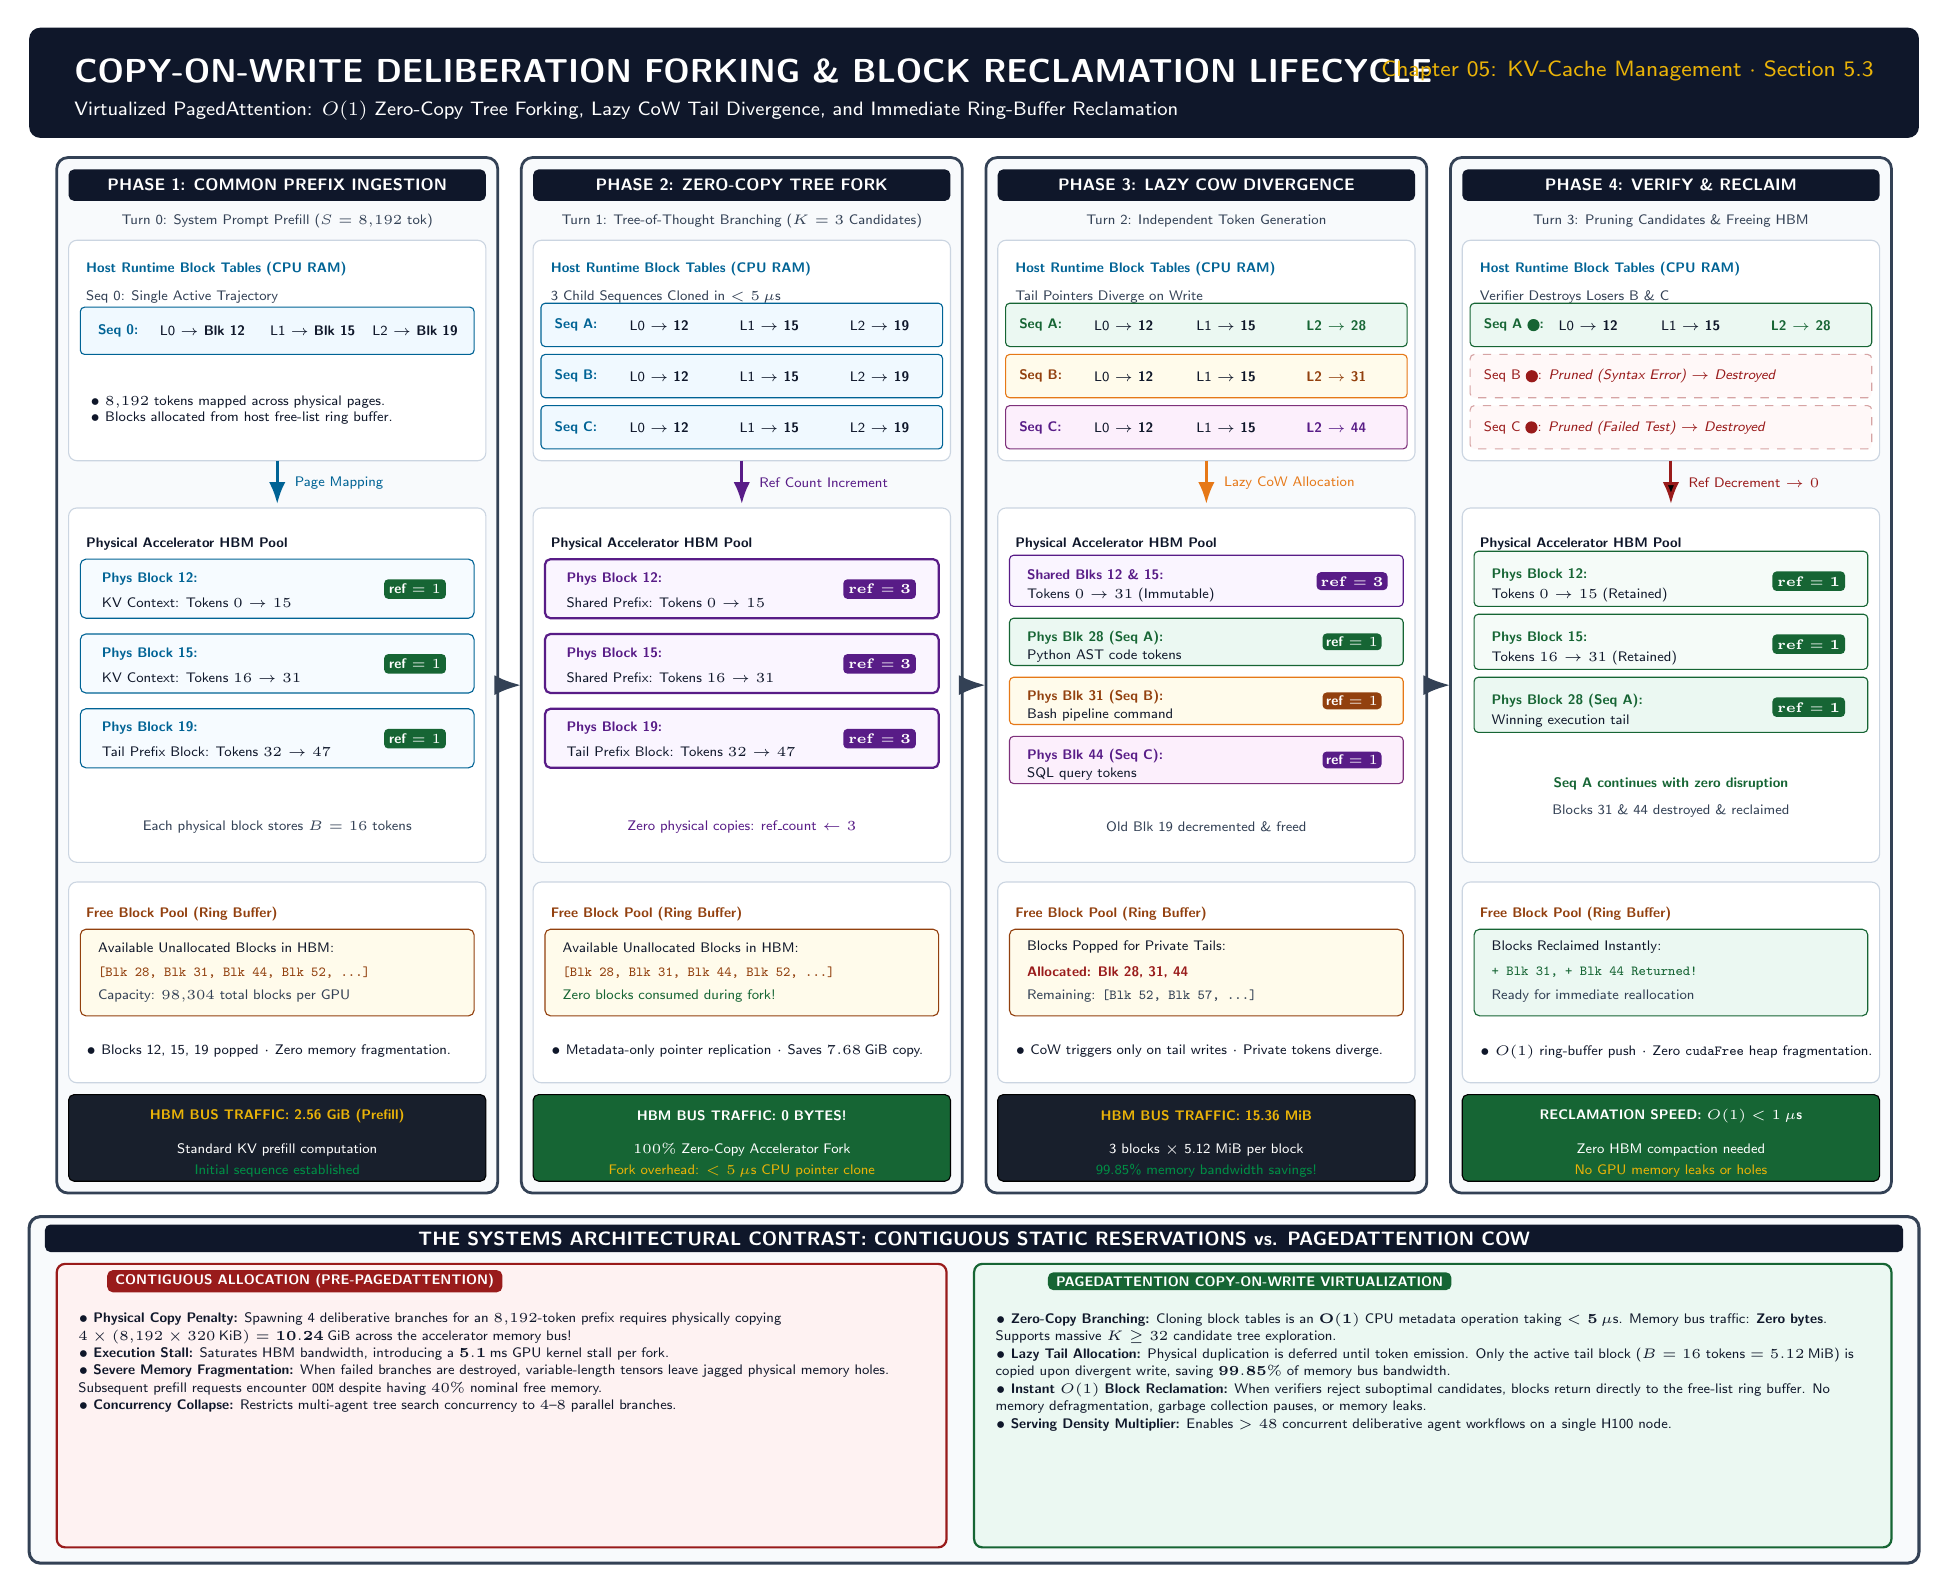
\begin{tikzpicture}[x=1cm, y=1cm]

% =============================================================================
% TOP TITLE BANNER (y: 18.6 to 20.0)
% =============================================================================
\draw[fill=DarkSlate, draw=none, rounded corners=4pt] (0, 18.6) rectangle (24.0, 20.0);
\node[anchor=west, font=\bfseries\large, text=white] at (0.45, 19.45) {
  COPY-ON-WRITE DELIBERATION FORKING \& BLOCK RECLAMATION LIFECYCLE
};
\node[anchor=east, font=\footnotesize, text=GoldPin] at (23.55, 19.45) {
  Chapter 05: KV-Cache Management $\cdot$ Section 5.3
};
\node[anchor=west, font=\scriptsize, text=white!85] at (0.45, 18.95) {
  Virtualized PagedAttention: $O(1)$ Zero-Copy Tree Forking, Lazy CoW Tail Divergence, and Immediate Ring-Buffer Reclamation
};

% =============================================================================
% 4 COLUMNS: THE TEMPORAL LIFECYCLE OF AN AGENT DELIBERATION FORK (y: 5.2 to 18.35)
% =============================================================================
% Col 1: x = 0.35 to 5.95 (Phase 1: Ingestion)
% Col 2: x = 6.25 to 11.85 (Phase 2: Tree Fork)
% Col 3: x = 12.15 to 17.75 (Phase 3: CoW Divergence)
% Col 4: x = 18.05 to 23.65 (Phase 4: Verification & Reclamation)

% -----------------------------------------------------------------------------
% COLUMN 1: PHASE 1 - COMMON PREFIX INGESTION (Turn 0)
% -----------------------------------------------------------------------------
\draw[draw=slatesteel, fill=coolparchment, line width=1.0pt, rounded corners=4pt] (0.35, 5.2) rectangle (5.95, 18.35);

% Header
\fill[DarkSlate, rounded corners=2pt] (0.5, 17.8) rectangle (5.8, 18.2);
\node[font=\bfseries\fontsize{6.2pt}{7.2pt}\selectfont, text=white] at (3.15, 18.0) {PHASE 1: COMMON PREFIX INGESTION};
\node[font=\fontsize{5.2pt}{6.2pt}\selectfont, text=slatesteel] at (3.15, 17.55) {Turn 0: System Prompt Prefill ($S = 8{,}192\text{ tok}$)};

% --- Logical Tables Tier (y: 14.50 to 17.30) ---
\draw[draw=CardBorder, fill=white, rounded corners=3pt] (0.5, 14.50) rectangle (5.8, 17.30);
\node[anchor=north west, font=\bfseries\fontsize{5.5pt}{6.5pt}\selectfont, text=BlueLine] at (0.6, 17.15) {Host Runtime Block Tables (CPU RAM)};
\node[anchor=north west, font=\fontsize{4.8pt}{5.8pt}\selectfont, text=slatesteel] at (0.6, 16.78) {Seq 0: Single Active Trajectory};

% Table row (concise L0, L1, L2 format)
\draw[draw=BlueLine, fill=BlueL0, rounded corners=1.5pt] (0.65, 15.85) rectangle (5.65, 16.45);
\node[anchor=west, font=\bfseries\fontsize{5.0pt}{6.0pt}\selectfont, text=BlueLine] at (0.75, 16.15) {Seq 0:};
\node[font=\fontsize{4.8pt}{5.8pt}\selectfont, text=DarkSlate] at (2.2, 16.15) {L0 $\to$ \textbf{Blk 12}};
\node[font=\fontsize{4.8pt}{5.8pt}\selectfont, text=DarkSlate] at (3.6, 16.15) {L1 $\to$ \textbf{Blk 15}};
\node[font=\fontsize{4.8pt}{5.8pt}\selectfont, text=DarkSlate] at (4.9, 16.15) {L2 $\to$ \textbf{Blk 19}};

\node[anchor=north west, font=\fontsize{4.8pt}{5.8pt}\selectfont, text=DarkSlate] at (0.65, 15.45) {
  \begin{minipage}{5.0cm}\raggedright
    $\bullet$ $8{,}192$ tokens mapped across physical pages.\\
    $\bullet$ Blocks allocated from host free-list ring buffer.
  \end{minipage}
};

% Arrow down to HBM (gutter: 14.50 to 13.90)
\draw[flow_arrow, draw=BlueLine] (3.15, 14.50) -- (3.15, 13.95);
\node[anchor=west, font=\fontsize{4.8pt}{5.8pt}\selectfont, text=BlueLine] at (3.25, 14.22) {Page Mapping};

% --- Physical HBM Block Pool Tier (y: 9.40 to 13.90, height: 4.5cm) ---
\draw[draw=CardBorder, fill=white, rounded corners=3pt] (0.5, 9.40) rectangle (5.8, 13.90);
\node[anchor=north west, font=\bfseries\fontsize{5.5pt}{6.5pt}\selectfont, text=DarkSlate] at (0.6, 13.65) {Physical Accelerator HBM Pool};

% Physical Block 12
\draw[draw=BlueLine, fill=BlueL0!60, rounded corners=2pt] (0.65, 12.50) rectangle (5.65, 13.25);
\node[anchor=west, font=\bfseries\fontsize{5.0pt}{6.0pt}\selectfont, text=BlueLine] at (0.8, 13.00) {Phys Block 12:};
\node[anchor=west, font=\fontsize{4.4pt}{5.4pt}\selectfont, text=DarkSlate] at (0.8, 12.70) {KV Context: Tokens $0 \to 15$};
\node[draw=none, fill=forestsage, rounded corners=1.5pt, text=white, font=\bfseries\fontsize{4.8pt}{5.8pt}\selectfont, inner sep=1.8pt] at (4.9, 12.87) {$\text{ref}=1$};

% Physical Block 15
\draw[draw=BlueLine, fill=BlueL0!60, rounded corners=2pt] (0.65, 11.55) rectangle (5.65, 12.30);
\node[anchor=west, font=\bfseries\fontsize{5.0pt}{6.0pt}\selectfont, text=BlueLine] at (0.8, 12.05) {Phys Block 15:};
\node[anchor=west, font=\fontsize{4.4pt}{5.4pt}\selectfont, text=DarkSlate] at (0.8, 11.75) {KV Context: Tokens $16 \to 31$};
\node[draw=none, fill=forestsage, rounded corners=1.5pt, text=white, font=\bfseries\fontsize{4.8pt}{5.8pt}\selectfont, inner sep=1.8pt] at (4.9, 11.92) {$\text{ref}=1$};

% Physical Block 19
\draw[draw=BlueLine, fill=BlueL0!60, rounded corners=2pt] (0.65, 10.60) rectangle (5.65, 11.35);
\node[anchor=west, font=\bfseries\fontsize{5.0pt}{6.0pt}\selectfont, text=BlueLine] at (0.8, 11.10) {Phys Block 19:};
\node[anchor=west, font=\fontsize{4.4pt}{5.4pt}\selectfont, text=DarkSlate] at (0.8, 10.80) {Tail Prefix Block: Tokens $32 \to 47$};
\node[draw=none, fill=forestsage, rounded corners=1.5pt, text=white, font=\bfseries\fontsize{4.8pt}{5.8pt}\selectfont, inner sep=1.8pt] at (4.9, 10.97) {$\text{ref}=1$};

\node[font=\fontsize{4.6pt}{5.6pt}\selectfont, text=slatesteel] at (3.15, 9.85) {Each physical block stores $B=16$ tokens};

% --- Free List Pool Tier (y: 6.60 to 9.15) ---
\draw[draw=CardBorder, fill=white, rounded corners=3pt] (0.5, 6.60) rectangle (5.8, 9.15);
\node[anchor=north west, font=\bfseries\fontsize{5.5pt}{6.5pt}\selectfont, text=warmochre] at (0.6, 8.95) {Free Block Pool (Ring Buffer)};

\draw[draw=warmochre, fill=OrangeL0, rounded corners=2pt] (0.65, 7.45) rectangle (5.65, 8.55);
\node[anchor=west, font=\fontsize{4.8pt}{5.8pt}\selectfont, text=DarkSlate] at (0.75, 8.32) {Available Unallocated Blocks in HBM:};
\node[anchor=west, font=\bfseries\fontsize{5.0pt}{6.0pt}\selectfont, text=warmochre] at (0.75, 8.00) {\texttt{[Blk 28, Blk 31, Blk 44, Blk 52, ...]}};
\node[anchor=west, font=\fontsize{4.6pt}{5.6pt}\selectfont, text=slatesteel] at (0.75, 7.70) {Capacity: $98{,}304$ total blocks per GPU};

\node[anchor=north west, font=\fontsize{4.6pt}{5.6pt}\selectfont, text=DarkSlate] at (0.6, 7.20) {
  \begin{minipage}{5.0cm}\raggedright
    $\bullet$ Blocks 12, 15, 19 popped $\cdot$ Zero memory fragmentation.
  \end{minipage}
};

% Bottom Status Badge
\draw[fill=ChipBlack, rounded corners=2pt] (0.5, 5.35) rectangle (5.8, 6.45);
\node[font=\bfseries\fontsize{5.2pt}{6.2pt}\selectfont, text=GoldPin] at (3.15, 6.18) {HBM BUS TRAFFIC: 2.56 GiB (Prefill)};
\node[font=\fontsize{4.8pt}{5.8pt}\selectfont, text=white!85] at (3.15, 5.75) {Standard KV prefill computation};
\node[font=\fontsize{4.6pt}{5.6pt}\selectfont, text=GreenLine] at (3.15, 5.48) {Initial sequence established};

% -----------------------------------------------------------------------------
% COLUMN 2: PHASE 2 - ZERO-COPY DELIBERATION FORK (Turn 1)
% -----------------------------------------------------------------------------
\draw[draw=slatesteel, fill=coolparchment, line width=1.0pt, rounded corners=4pt] (6.25, 5.2) rectangle (11.85, 18.35);

% Header
\fill[DarkSlate, rounded corners=2pt] (6.4, 17.8) rectangle (11.7, 18.2);
\node[font=\bfseries\fontsize{6.2pt}{7.2pt}\selectfont, text=white] at (9.05, 18.0) {PHASE 2: ZERO-COPY TREE FORK};
\node[font=\fontsize{5.2pt}{6.2pt}\selectfont, text=slatesteel] at (9.05, 17.55) {Turn 1: Tree-of-Thought Branching ($K=3$ Candidates)};

% --- Logical Tables Tier (y: 14.50 to 17.30) ---
\draw[draw=CardBorder, fill=white, rounded corners=3pt] (6.4, 14.50) rectangle (11.7, 17.30);
\node[anchor=north west, font=\bfseries\fontsize{5.5pt}{6.5pt}\selectfont, text=BlueLine] at (6.5, 17.15) {Host Runtime Block Tables (CPU RAM)};
\node[anchor=north west, font=\fontsize{4.8pt}{5.8pt}\selectfont, text=slatesteel] at (6.5, 16.78) {3 Child Sequences Cloned in $<5\,\mu\text{s}$};

% Seq A
\draw[draw=BlueLine, fill=BlueL0, rounded corners=1.5pt] (6.5, 15.95) rectangle (11.6, 16.50);
\node[anchor=west, font=\bfseries\fontsize{4.8pt}{5.8pt}\selectfont, text=BlueLine] at (6.55, 16.22) {Seq A:};
\node[font=\fontsize{4.6pt}{5.6pt}\selectfont, text=DarkSlate] at (8.0, 16.22) {L0 $\to$ \textbf{12}};
\node[font=\fontsize{4.6pt}{5.6pt}\selectfont, text=DarkSlate] at (9.4, 16.22) {L1 $\to$ \textbf{15}};
\node[font=\fontsize{4.6pt}{5.6pt}\selectfont, text=DarkSlate] at (10.8, 16.22) {L2 $\to$ \textbf{19}};

% Seq B
\draw[draw=BlueLine, fill=BlueL0, rounded corners=1.5pt] (6.5, 15.30) rectangle (11.6, 15.85);
\node[anchor=west, font=\bfseries\fontsize{4.8pt}{5.8pt}\selectfont, text=BlueLine] at (6.55, 15.57) {Seq B:};
\node[font=\fontsize{4.6pt}{5.6pt}\selectfont, text=DarkSlate] at (8.0, 15.57) {L0 $\to$ \textbf{12}};
\node[font=\fontsize{4.6pt}{5.6pt}\selectfont, text=DarkSlate] at (9.4, 15.57) {L1 $\to$ \textbf{15}};
\node[font=\fontsize{4.6pt}{5.6pt}\selectfont, text=DarkSlate] at (10.8, 15.57) {L2 $\to$ \textbf{19}};

% Seq C
\draw[draw=BlueLine, fill=BlueL0, rounded corners=1.5pt] (6.5, 14.65) rectangle (11.6, 15.20);
\node[anchor=west, font=\bfseries\fontsize{4.8pt}{5.8pt}\selectfont, text=BlueLine] at (6.55, 14.92) {Seq C:};
\node[font=\fontsize{4.6pt}{5.6pt}\selectfont, text=DarkSlate] at (8.0, 14.92) {L0 $\to$ \textbf{12}};
\node[font=\fontsize{4.6pt}{5.6pt}\selectfont, text=DarkSlate] at (9.4, 14.92) {L1 $\to$ \textbf{15}};
\node[font=\fontsize{4.6pt}{5.6pt}\selectfont, text=DarkSlate] at (10.8, 14.92) {L2 $\to$ \textbf{19}};

% Arrow down to HBM (gutter: 14.50 to 13.90)
\draw[flow_arrow, draw=amethyst] (9.05, 14.50) -- (9.05, 13.95);
\node[anchor=west, font=\fontsize{4.8pt}{5.8pt}\selectfont, text=amethyst] at (9.15, 14.22) {Ref Count Increment};

% --- Physical HBM Block Pool Tier (y: 9.40 to 13.90) ---
\draw[draw=CardBorder, fill=white, rounded corners=3pt] (6.4, 9.40) rectangle (11.7, 13.90);
\node[anchor=north west, font=\bfseries\fontsize{5.5pt}{6.5pt}\selectfont, text=DarkSlate] at (6.5, 13.65) {Physical Accelerator HBM Pool};

% Physical Block 12
\draw[draw=amethyst, fill=amethystL0, rounded corners=2pt, line width=0.8pt] (6.55, 12.50) rectangle (11.55, 13.25);
\node[anchor=west, font=\bfseries\fontsize{5.0pt}{6.0pt}\selectfont, text=amethyst] at (6.7, 13.00) {Phys Block 12:};
\node[anchor=west, font=\fontsize{4.4pt}{5.4pt}\selectfont, text=DarkSlate] at (6.7, 12.70) {Shared Prefix: Tokens $0 \to 15$};
\node[draw=none, fill=amethyst, rounded corners=1.5pt, text=white, font=\bfseries\fontsize{5.0pt}{6.0pt}\selectfont, inner sep=1.8pt] at (10.8, 12.87) {$\mathbf{ref=3}$};

% Physical Block 15
\draw[draw=amethyst, fill=amethystL0, rounded corners=2pt, line width=0.8pt] (6.55, 11.55) rectangle (11.55, 12.30);
\node[anchor=west, font=\bfseries\fontsize{5.0pt}{6.0pt}\selectfont, text=amethyst] at (6.7, 12.05) {Phys Block 15:};
\node[anchor=west, font=\fontsize{4.4pt}{5.4pt}\selectfont, text=DarkSlate] at (6.7, 11.75) {Shared Prefix: Tokens $16 \to 31$};
\node[draw=none, fill=amethyst, rounded corners=1.5pt, text=white, font=\bfseries\fontsize{5.0pt}{6.0pt}\selectfont, inner sep=1.8pt] at (10.8, 11.92) {$\mathbf{ref=3}$};

% Physical Block 19
\draw[draw=amethyst, fill=amethystL0, rounded corners=2pt, line width=0.8pt] (6.55, 10.60) rectangle (11.55, 11.35);
\node[anchor=west, font=\bfseries\fontsize{5.0pt}{6.0pt}\selectfont, text=amethyst] at (6.7, 11.10) {Phys Block 19:};
\node[anchor=west, font=\fontsize{4.4pt}{5.4pt}\selectfont, text=DarkSlate] at (6.7, 10.80) {Tail Prefix Block: Tokens $32 \to 47$};
\node[draw=none, fill=amethyst, rounded corners=1.5pt, text=white, font=\bfseries\fontsize{5.0pt}{6.0pt}\selectfont, inner sep=1.8pt] at (10.8, 10.97) {$\mathbf{ref=3}$};

\node[font=\fontsize{4.6pt}{5.6pt}\selectfont, text=amethyst] at (9.05, 9.85) {Zero physical copies: $\text{ref\_count} \leftarrow 3$};

% --- Free List Pool Tier (y: 6.60 to 9.15) ---
\draw[draw=CardBorder, fill=white, rounded corners=3pt] (6.4, 6.60) rectangle (11.7, 9.15);
\node[anchor=north west, font=\bfseries\fontsize{5.5pt}{6.5pt}\selectfont, text=warmochre] at (6.5, 8.95) {Free Block Pool (Ring Buffer)};

\draw[draw=warmochre, fill=OrangeL0, rounded corners=2pt] (6.55, 7.45) rectangle (11.55, 8.55);
\node[anchor=west, font=\fontsize{4.8pt}{5.8pt}\selectfont, text=DarkSlate] at (6.65, 8.32) {Available Unallocated Blocks in HBM:};
\node[anchor=west, font=\bfseries\fontsize{5.0pt}{6.0pt}\selectfont, text=warmochre] at (6.65, 8.00) {\texttt{[Blk 28, Blk 31, Blk 44, Blk 52, ...]}};
\node[anchor=west, font=\fontsize{4.6pt}{5.6pt}\selectfont, text=forestsage] at (6.65, 7.70) {Zero blocks consumed during fork!};

\node[anchor=north west, font=\fontsize{4.6pt}{5.6pt}\selectfont, text=DarkSlate] at (6.5, 7.20) {
  \begin{minipage}{5.0cm}\raggedright
    $\bullet$ Metadata-only pointer replication $\cdot$ Saves $7.68\,\text{GiB}$ copy.
  \end{minipage}
};

% Bottom Status Badge
\draw[fill=forestsage, rounded corners=2pt] (6.4, 5.35) rectangle (11.7, 6.45);
\node[font=\bfseries\fontsize{5.5pt}{6.5pt}\selectfont, text=white] at (9.05, 6.18) {HBM BUS TRAFFIC: 0 BYTES!};
\node[font=\fontsize{4.8pt}{5.8pt}\selectfont, text=white!95] at (9.05, 5.75) {$100\%$ Zero-Copy Accelerator Fork};
\node[font=\fontsize{4.6pt}{5.6pt}\selectfont, text=GoldPin] at (9.05, 5.48) {Fork overhead: $<5\,\mu\text{s}$ CPU pointer clone};

% -----------------------------------------------------------------------------
% COLUMN 3: PHASE 3 - LAZY COW DIVERGENCE (Turn 2)
% -----------------------------------------------------------------------------
\draw[draw=slatesteel, fill=coolparchment, line width=1.0pt, rounded corners=4pt] (12.15, 5.2) rectangle (17.75, 18.35);

% Header
\fill[DarkSlate, rounded corners=2pt] (12.3, 17.8) rectangle (17.6, 18.2);
\node[font=\bfseries\fontsize{6.2pt}{7.2pt}\selectfont, text=white] at (14.95, 18.0) {PHASE 3: LAZY COW DIVERGENCE};
\node[font=\fontsize{5.2pt}{6.2pt}\selectfont, text=slatesteel] at (14.95, 17.55) {Turn 2: Independent Token Generation};

% --- Logical Tables Tier (y: 14.50 to 17.30) ---
\draw[draw=CardBorder, fill=white, rounded corners=3pt] (12.3, 14.50) rectangle (17.6, 17.30);
\node[anchor=north west, font=\bfseries\fontsize{5.5pt}{6.5pt}\selectfont, text=BlueLine] at (12.4, 17.15) {Host Runtime Block Tables (CPU RAM)};
\node[anchor=north west, font=\fontsize{4.8pt}{5.8pt}\selectfont, text=slatesteel] at (12.4, 16.78) {Tail Pointers Diverge on Write};

% Seq A
\draw[draw=forestsage, fill=GreenL0, rounded corners=1.5pt] (12.4, 15.95) rectangle (17.5, 16.50);
\node[anchor=west, font=\bfseries\fontsize{4.8pt}{5.8pt}\selectfont, text=forestsage] at (12.45, 16.22) {Seq A:};
\node[font=\fontsize{4.6pt}{5.6pt}\selectfont, text=DarkSlate] at (13.9, 16.22) {L0 $\to$ \textbf{12}};
\node[font=\fontsize{4.6pt}{5.6pt}\selectfont, text=DarkSlate] at (15.2, 16.22) {L1 $\to$ \textbf{15}};
\node[font=\bfseries\fontsize{4.6pt}{5.6pt}\selectfont, text=forestsage] at (16.6, 16.22) {L2 $\to$ \textbf{28}};

% Seq B
\draw[draw=OrangeLine, fill=OrangeL0, rounded corners=1.5pt] (12.4, 15.30) rectangle (17.5, 15.85);
\node[anchor=west, font=\bfseries\fontsize{4.8pt}{5.8pt}\selectfont, text=warmochre] at (12.45, 15.57) {Seq B:};
\node[font=\fontsize{4.6pt}{5.6pt}\selectfont, text=DarkSlate] at (13.9, 15.57) {L0 $\to$ \textbf{12}};
\node[font=\fontsize{4.6pt}{5.6pt}\selectfont, text=DarkSlate] at (15.2, 15.57) {L1 $\to$ \textbf{15}};
\node[font=\bfseries\fontsize{4.6pt}{5.6pt}\selectfont, text=warmochre] at (16.6, 15.57) {L2 $\to$ \textbf{31}};

% Seq C
\draw[draw=VioletLine, fill=VioletL!40, rounded corners=1.5pt] (12.4, 14.65) rectangle (17.5, 15.20);
\node[anchor=west, font=\bfseries\fontsize{4.8pt}{5.8pt}\selectfont, text=amethyst] at (12.45, 14.92) {Seq C:};
\node[font=\fontsize{4.6pt}{5.6pt}\selectfont, text=DarkSlate] at (13.9, 14.92) {L0 $\to$ \textbf{12}};
\node[font=\fontsize{4.6pt}{5.6pt}\selectfont, text=DarkSlate] at (15.2, 14.92) {L1 $\to$ \textbf{15}};
\node[font=\bfseries\fontsize{4.6pt}{5.6pt}\selectfont, text=amethyst] at (16.6, 14.92) {L2 $\to$ \textbf{44}};

% Arrow down to HBM (gutter: 14.50 to 13.90)
\draw[flow_arrow, draw=OrangeLine] (14.95, 14.50) -- (14.95, 13.95);
\node[anchor=west, font=\fontsize{4.8pt}{5.8pt}\selectfont, text=OrangeLine] at (15.05, 14.22) {Lazy CoW Allocation};

% --- Physical HBM Block Pool Tier (y: 9.40 to 13.90) ---
\draw[draw=CardBorder, fill=white, rounded corners=3pt] (12.3, 9.40) rectangle (17.6, 13.90);
\node[anchor=north west, font=\bfseries\fontsize{5.5pt}{6.5pt}\selectfont, text=DarkSlate] at (12.4, 13.65) {Physical Accelerator HBM Pool};

% Shared Prefix Blocks 12 & 15
\draw[draw=amethyst, fill=amethystL0, rounded corners=1.5pt] (12.45, 12.65) rectangle (17.45, 13.30);
\node[anchor=west, font=\bfseries\fontsize{4.8pt}{5.8pt}\selectfont, text=amethyst] at (12.55, 13.05) {Shared Blks 12 \& 15:};
\node[anchor=west, font=\fontsize{4.4pt}{5.4pt}\selectfont, text=DarkSlate] at (12.55, 12.80) {Tokens $0 \to 31$ (Immutable)};
\node[draw=none, fill=amethyst, rounded corners=1.5pt, text=white, font=\bfseries\fontsize{4.8pt}{5.8pt}\selectfont, inner sep=1.5pt] at (16.8, 12.97) {$\mathbf{ref=3}$};

% Private Divergent Blocks
\draw[draw=forestsage, fill=GreenL0, rounded corners=1.5pt] (12.45, 11.90) rectangle (17.45, 12.50);
\node[anchor=west, font=\bfseries\fontsize{4.8pt}{5.8pt}\selectfont, text=forestsage] at (12.55, 12.25) {Phys Blk 28 (Seq A):};
\node[anchor=west, font=\fontsize{4.4pt}{5.4pt}\selectfont, text=DarkSlate] at (12.55, 12.02) {Python AST code tokens};
\node[draw=none, fill=forestsage, rounded corners=1.5pt, text=white, font=\bfseries\fontsize{4.6pt}{5.6pt}\selectfont, inner sep=1.3pt] at (16.8, 12.20) {$\text{ref}=1$};

\draw[draw=OrangeLine, fill=OrangeL0, rounded corners=1.5pt] (12.45, 11.15) rectangle (17.45, 11.75);
\node[anchor=west, font=\bfseries\fontsize{4.8pt}{5.8pt}\selectfont, text=warmochre] at (12.55, 11.50) {Phys Blk 31 (Seq B):};
\node[anchor=west, font=\fontsize{4.4pt}{5.4pt}\selectfont, text=DarkSlate] at (12.55, 11.27) {Bash pipeline command};
\node[draw=none, fill=warmochre, rounded corners=1.5pt, text=white, font=\bfseries\fontsize{4.6pt}{5.6pt}\selectfont, inner sep=1.3pt] at (16.8, 11.45) {$\text{ref}=1$};

\draw[draw=VioletLine, fill=VioletL!40, rounded corners=1.5pt] (12.45, 10.40) rectangle (17.45, 11.00);
\node[anchor=west, font=\bfseries\fontsize{4.8pt}{5.8pt}\selectfont, text=amethyst] at (12.55, 10.75) {Phys Blk 44 (Seq C):};
\node[anchor=west, font=\fontsize{4.4pt}{5.4pt}\selectfont, text=DarkSlate] at (12.55, 10.52) {SQL query tokens};
\node[draw=none, fill=amethyst, rounded corners=1.5pt, text=white, font=\bfseries\fontsize{4.6pt}{5.6pt}\selectfont, inner sep=1.3pt] at (16.8, 10.70) {$\text{ref}=1$};

\node[font=\fontsize{4.6pt}{5.6pt}\selectfont, text=slatesteel] at (14.95, 9.85) {Old Blk 19 decremented \& freed};

% --- Free List Pool Tier (y: 6.60 to 9.15) ---
\draw[draw=CardBorder, fill=white, rounded corners=3pt] (12.3, 6.60) rectangle (17.6, 9.15);
\node[anchor=north west, font=\bfseries\fontsize{5.5pt}{6.5pt}\selectfont, text=warmochre] at (12.4, 8.95) {Free Block Pool (Ring Buffer)};

\draw[draw=warmochre, fill=OrangeL0, rounded corners=2pt] (12.45, 7.45) rectangle (17.45, 8.55);
\node[anchor=west, font=\fontsize{4.8pt}{5.8pt}\selectfont, text=DarkSlate] at (12.55, 8.32) {Blocks Popped for Private Tails:};
\node[anchor=west, font=\bfseries\fontsize{5.0pt}{6.0pt}\selectfont, text=deepburgundy] at (12.55, 8.00) {Allocated: Blk 28, 31, 44};
\node[anchor=west, font=\fontsize{4.6pt}{5.6pt}\selectfont, text=slatesteel] at (12.55, 7.70) {Remaining: \texttt{[Blk 52, Blk 57, ...]}};

\node[anchor=north west, font=\fontsize{4.6pt}{5.6pt}\selectfont, text=DarkSlate] at (12.4, 7.20) {
  \begin{minipage}{5.0cm}\raggedright
    $\bullet$ CoW triggers only on tail writes $\cdot$ Private tokens diverge.
  \end{minipage}
};

% Bottom Status Badge
\draw[fill=ChipBlack, rounded corners=2pt] (12.3, 5.35) rectangle (17.6, 6.45);
\node[font=\bfseries\fontsize{5.2pt}{6.2pt}\selectfont, text=GoldPin] at (14.95, 6.18) {HBM BUS TRAFFIC: 15.36 MiB};
\node[font=\fontsize{4.8pt}{5.8pt}\selectfont, text=white!85] at (14.95, 5.75) {3 blocks $\times$ 5.12 MiB per block};
\node[font=\fontsize{4.6pt}{5.6pt}\selectfont, text=GreenLine] at (14.95, 5.48) {99.85\% memory bandwidth savings!};

% -----------------------------------------------------------------------------
% COLUMN 4: PHASE 4 - VERIFICATION & RECLAMATION (Turn 3)
% -----------------------------------------------------------------------------
\draw[draw=slatesteel, fill=coolparchment, line width=1.0pt, rounded corners=4pt] (18.05, 5.2) rectangle (23.65, 18.35);

% Header
\fill[DarkSlate, rounded corners=2pt] (18.2, 17.8) rectangle (23.5, 18.2);
\node[font=\bfseries\fontsize{6.2pt}{7.2pt}\selectfont, text=white] at (20.85, 18.0) {PHASE 4: VERIFY \& RECLAIM};
\node[font=\fontsize{5.2pt}{6.2pt}\selectfont, text=slatesteel] at (20.85, 17.55) {Turn 3: Pruning Candidates \& Freeing HBM};

% --- Logical Tables Tier (y: 14.50 to 17.30) ---
\draw[draw=CardBorder, fill=white, rounded corners=3pt] (18.2, 14.50) rectangle (23.5, 17.30);
\node[anchor=north west, font=\bfseries\fontsize{5.5pt}{6.5pt}\selectfont, text=BlueLine] at (18.3, 17.15) {Host Runtime Block Tables (CPU RAM)};
\node[anchor=north west, font=\fontsize{4.8pt}{5.8pt}\selectfont, text=slatesteel] at (18.3, 16.78) {Verifier Destroys Losers B \& C};

% Seq A (Winner)
\draw[draw=forestsage, fill=GreenL0, rounded corners=1.5pt] (18.3, 15.95) rectangle (23.4, 16.50);
\node[anchor=west, font=\bfseries\fontsize{4.8pt}{5.8pt}\selectfont, text=forestsage] at (18.35, 16.22) {Seq A \greenpass:};
\node[font=\fontsize{4.6pt}{5.6pt}\selectfont, text=DarkSlate] at (19.8, 16.22) {L0 $\to$ \textbf{12}};
\node[font=\fontsize{4.6pt}{5.6pt}\selectfont, text=DarkSlate] at (21.1, 16.22) {L1 $\to$ \textbf{15}};
\node[font=\bfseries\fontsize{4.6pt}{5.6pt}\selectfont, text=forestsage] at (22.5, 16.22) {L2 $\to$ \textbf{28}};

% Seq B (Killed)
\draw[draw=deepburgundy!40, fill=RedL0!50, rounded corners=1.5pt, dashed] (18.3, 15.30) rectangle (23.4, 15.85);
\node[anchor=west, font=\fontsize{4.6pt}{5.6pt}\selectfont, text=deepburgundy] at (18.35, 15.57) {Seq B \redfail: \textit{Pruned (Syntax Error) $\to$ Destroyed}};

% Seq C (Killed)
\draw[draw=deepburgundy!40, fill=RedL0!50, rounded corners=1.5pt, dashed] (18.3, 14.65) rectangle (23.4, 15.20);
\node[anchor=west, font=\fontsize{4.6pt}{5.6pt}\selectfont, text=deepburgundy] at (18.35, 14.92) {Seq C \redfail: \textit{Pruned (Failed Test) $\to$ Destroyed}};

% Arrow down to HBM (gutter: 14.50 to 13.90)
\draw[flow_arrow, draw=deepburgundy] (20.85, 14.50) -- (20.85, 13.95);
\node[anchor=west, font=\fontsize{4.8pt}{5.8pt}\selectfont, text=deepburgundy] at (20.95, 14.22) {Ref Decrement $\to 0$};

% --- Physical HBM Block Pool Tier (y: 9.40 to 13.90) ---
\draw[draw=CardBorder, fill=white, rounded corners=3pt] (18.2, 9.40) rectangle (23.5, 13.90);
\node[anchor=north west, font=\bfseries\fontsize{5.5pt}{6.5pt}\selectfont, text=DarkSlate] at (18.3, 13.65) {Physical Accelerator HBM Pool};

% Physical Block 12
\draw[draw=forestsage, fill=GreenL0!50, rounded corners=1.5pt] (18.35, 12.65) rectangle (23.35, 13.35);
\node[anchor=west, font=\bfseries\fontsize{4.8pt}{5.8pt}\selectfont, text=forestsage] at (18.45, 13.05) {Phys Block 12:};
\node[anchor=west, font=\fontsize{4.4pt}{5.4pt}\selectfont, text=DarkSlate] at (18.45, 12.80) {Tokens $0 \to 15$ (Retained)};
\node[draw=none, fill=forestsage, rounded corners=1.5pt, text=white, font=\bfseries\fontsize{4.8pt}{5.8pt}\selectfont, inner sep=1.8pt] at (22.6, 12.97) {$\mathbf{ref=1}$};

% Physical Block 15
\draw[draw=forestsage, fill=GreenL0!50, rounded corners=1.5pt] (18.35, 11.85) rectangle (23.35, 12.55);
\node[anchor=west, font=\bfseries\fontsize{4.8pt}{5.8pt}\selectfont, text=forestsage] at (18.45, 12.25) {Phys Block 15:};
\node[anchor=west, font=\fontsize{4.4pt}{5.4pt}\selectfont, text=DarkSlate] at (18.45, 12.00) {Tokens $16 \to 31$ (Retained)};
\node[draw=none, fill=forestsage, rounded corners=1.5pt, text=white, font=\bfseries\fontsize{4.8pt}{5.8pt}\selectfont, inner sep=1.8pt] at (22.6, 12.17) {$\mathbf{ref=1}$};

% Physical Block 28
\draw[draw=forestsage, fill=GreenL0, rounded corners=1.5pt] (18.35, 11.05) rectangle (23.35, 11.75);
\node[anchor=west, font=\bfseries\fontsize{4.8pt}{5.8pt}\selectfont, text=forestsage] at (18.45, 11.45) {Phys Block 28 (Seq A):};
\node[anchor=west, font=\fontsize{4.4pt}{5.4pt}\selectfont, text=DarkSlate] at (18.45, 11.20) {Winning execution tail};
\node[draw=none, fill=forestsage, rounded corners=1.5pt, text=white, font=\bfseries\fontsize{4.8pt}{5.8pt}\selectfont, inner sep=1.8pt] at (22.6, 11.37) {$\mathbf{ref=1}$};

\node[font=\bfseries\fontsize{4.8pt}{5.8pt}\selectfont, text=forestsage] at (20.85, 10.40) {Seq A continues with zero disruption};
\node[font=\fontsize{4.4pt}{5.4pt}\selectfont, text=slatesteel] at (20.85, 10.05) {Blocks 31 \& 44 destroyed \& reclaimed};

% --- Free List Pool Tier (y: 6.60 to 9.15) ---
\draw[draw=CardBorder, fill=white, rounded corners=3pt] (18.2, 6.60) rectangle (23.5, 9.15);
\node[anchor=north west, font=\bfseries\fontsize{5.5pt}{6.5pt}\selectfont, text=warmochre] at (18.3, 8.95) {Free Block Pool (Ring Buffer)};

\draw[draw=forestsage, fill=GreenL0, rounded corners=2pt] (18.35, 7.45) rectangle (23.35, 8.55);
\node[anchor=west, font=\fontsize{4.8pt}{5.8pt}\selectfont, text=DarkSlate] at (18.45, 8.32) {Blocks Reclaimed Instantly:};
\node[anchor=west, font=\bfseries\fontsize{5.0pt}{6.0pt}\selectfont, text=forestsage] at (18.45, 8.00) {\texttt{+ Blk 31, + Blk 44 Returned!}};
\node[anchor=west, font=\fontsize{4.6pt}{5.6pt}\selectfont, text=slatesteel] at (18.45, 7.70) {Ready for immediate reallocation};

\node[anchor=north west, font=\fontsize{4.6pt}{5.6pt}\selectfont, text=DarkSlate] at (18.3, 7.20) {
  \begin{minipage}{5.0cm}\raggedright
    $\bullet$ $O(1)$ ring-buffer push $\cdot$ Zero \texttt{cudaFree} heap fragmentation.
  \end{minipage}
};

% Bottom Status Badge
\draw[fill=forestsage, rounded corners=2pt] (18.2, 5.35) rectangle (23.5, 6.45);
\node[font=\bfseries\fontsize{5.2pt}{6.2pt}\selectfont, text=white] at (20.85, 6.18) {RECLAMATION SPEED: $O(1)$ $<1\,\mu\text{s}$};
\node[font=\fontsize{4.8pt}{5.8pt}\selectfont, text=white!95] at (20.85, 5.75) {Zero HBM compaction needed};
\node[font=\fontsize{4.6pt}{5.6pt}\selectfont, text=GoldPin] at (20.85, 5.48) {No GPU memory leaks or holes};

% Horizontal Flow Arrows between Columns
\draw[flow_arrow_thick, draw=slatesteel] (5.95, 11.65) -- (6.25, 11.65);
\draw[flow_arrow_thick, draw=slatesteel] (11.85, 11.65) -- (12.15, 11.65);
\draw[flow_arrow_thick, draw=slatesteel] (17.75, 11.65) -- (18.05, 11.65);

% =============================================================================
% BOTTOM TIER: CONTIGUOUS ALLOCATION vs. PAGEDATTENTION COW (y: 0.5 to 4.9)
% =============================================================================
\draw[draw=slatesteel, fill=coolparchment, line width=1.1pt, rounded corners=4pt] (0, 0.5) rectangle (24.0, 4.9);

% Header Bar
\fill[DarkSlate, rounded corners=2pt] (0.2, 4.45) rectangle (23.8, 4.8);
\node[font=\bfseries\fontsize{6.8pt}{8.2pt}\selectfont, text=white] at (12.0, 4.62) {
  THE SYSTEMS ARCHITECTURAL CONTRAST: CONTIGUOUS STATIC RESERVATIONS vs. PAGEDATTENTION COW
};

% --- Left Box: Contiguous Allocation Pathology (x: 0.35 to 11.65) ---
\draw[draw=deepburgundy, fill=RedL0, rounded corners=3pt, line width=0.8pt] (0.35, 0.7) rectangle (11.65, 4.3);
\node[draw=none, fill=deepburgundy, rounded corners=2pt, inner xsep=3pt, inner ysep=1.5pt, font=\bfseries\fontsize{5.5pt}{6.5pt}\selectfont, text=white] at (3.5, 4.08) {CONTIGUOUS ALLOCATION (PRE-PAGEDATTENTION)};

\node[anchor=north west, font=\fontsize{5.0pt}{6.3pt}\selectfont, text=DarkSlate] at (0.5, 3.8) {
  \begin{minipage}{10.8cm}\raggedright
    $\bullet$ \textbf{Physical Copy Penalty:} Spawning 4 deliberative branches for an $8{,}192$-token prefix requires physically copying $4 \times (8{,}192 \times 320\,\text{KiB}) = \mathbf{10.24\,\text{GiB}}$ across the accelerator memory bus!\\
    $\bullet$ \textbf{Execution Stall:} Saturates HBM bandwidth, introducing a $\mathbf{5.1\,\text{ms}}$ GPU kernel stall per fork.\\
    $\bullet$ \textbf{Severe Memory Fragmentation:} When failed branches are destroyed, variable-length tensors leave jagged physical memory holes. Subsequent prefill requests encounter \texttt{OOM} despite having $40\%$ nominal free memory.\\
    $\bullet$ \textbf{Concurrency Collapse:} Restricts multi-agent tree search concurrency to $4\text{--}8$ parallel branches.
  \end{minipage}
};

% --- Right Box: PagedAttention CoW Advantages (x: 12.00 to 23.65) ---
\draw[draw=forestsage, fill=GreenL0, rounded corners=3pt, line width=0.8pt] (12.0, 0.7) rectangle (23.65, 4.3);
\node[draw=none, fill=forestsage, rounded corners=2pt, inner xsep=3pt, inner ysep=1.5pt, font=\bfseries\fontsize{5.5pt}{6.5pt}\selectfont, text=white] at (15.5, 4.08) {PAGEDATTENTION COPY-ON-WRITE VIRTUALIZATION};

\node[anchor=north west, font=\fontsize{5.0pt}{6.3pt}\selectfont, text=DarkSlate] at (12.15, 3.8) {
  \begin{minipage}{11.1cm}\raggedright
    $\bullet$ \textbf{Zero-Copy Branching:} Cloning block tables is an $\mathbf{O(1)}$ CPU metadata operation taking $<\mathbf{5\,\mu\text{s}}$. Memory bus traffic: \textbf{Zero bytes}. Supports massive $K \ge 32$ candidate tree exploration.\\
    $\bullet$ \textbf{Lazy Tail Allocation:} Physical duplication is deferred until token emission. Only the active tail block ($B=16$ tokens $= 5.12\,\text{MiB}$) is copied upon divergent write, saving $\mathbf{99.85\%}$ of memory bus bandwidth.\\
    $\bullet$ \textbf{Instant $O(1)$ Block Reclamation:} When verifiers reject suboptimal candidates, blocks return directly to the free-list ring buffer. No memory defragmentation, garbage collection pauses, or memory leaks.\\
    $\bullet$ \textbf{Serving Density Multiplier:} Enables $>48$ concurrent deliberative agent workflows on a single H100 node.
  \end{minipage}
};

\end{tikzpicture}
\end{document}
